
\documentclass{article} % For LaTeX2e
\usepackage{iclr2027_conference,times}

% Optional math commands from https://github.com/goodfeli/dlbook_notation.
\input{math_commands.tex}
% Shared notation. Edit here rather than repeating in the body.
\newcommand{\znow}{z_{\mathrm{now}}}
\newcommand{\zg}{z_{g}}
\newcommand{\planlen}{25}
\newcommand{\Fk}{F^{k}}
\newcommand{\Bk}{B^{k}}


\usepackage{url}
\usepackage{amsmath,amssymb}
\usepackage{algorithm}
\usepackage{algpseudocode}

% Figures/tables only; do not edit iclr2027_conference.sty.
\usepackage{graphicx}
\usepackage{booktabs}
\usepackage{hyperref}


\title{Horizon-Aligned Scoring: A Longer View for\\
Short-Horizon World-Model Planning}

% Authors must not appear in the submitted version. They should be hidden
% as long as the \iclrfinalcopy macro remains commented out below.
% Non-anonymous submissions will be rejected without review.

\author{Yuan Ben \\
Institution \\
Address \\
\texttt{email}
}

% The \author macro works with any number of authors. There are two commands
% used to separate the names and addresses of multiple authors: \And and \AND.
%
% Using \And between authors leaves it to \LaTeX{} to determine where to break
% the lines. Using \AND forces a linebreak at that point. So, if \LaTeX{}
% puts 3 of 4 authors names on the first line, and the last on the second
% line, try using \AND instead of \And before the third author name.

\newcommand{\fix}{\marginpar{FIX}}
\newcommand{\new}{\marginpar{NEW}}

%\iclrfinalcopy % Uncomment for camera-ready version, but NOT for submission.
\begin{document}


\maketitle

\begin{abstract}
Visual world-model planners evaluate candidate actions through short
latent rollouts, while their goals often require progress over a longer
time scale. Direct endpoint-to-goal distance can undervalue actions
whose benefits emerge after the current planning span. We introduce
Horizon-Aligned Scoring (HAS), which gives each short-rollout endpoint
a longer-horizon scoring view. HAS learns an action-free Forward
imaginer from local latent transitions and recursively extends the
action-conditioned endpoint before computing its distance to the
visual goal. The recursion depth follows the remaining temporal gap
and decreases as execution advances. Across ten paired evaluation
groups on PushT, TwoRoom, and Reacher, HAS improves mean success at
every evaluated goal offset beyond the default planning span.
It raises PushT success from $42.8\%$ to $67.8\%$ at offset $50$ and
TwoRoom success from $16.4\%$ to $70.4\%$ at offset $100$.
HAS also exceeds the evaluated longer-span LeWM configuration at all
offsets of $50$ steps or more, while a fixed-depth comparison highlights
the importance of adapting the extension during execution.
These results establish the scoring time scale as an effective design
dimension for short-horizon world-model planning.
\end{abstract}

\section{Introduction}
\label{sec:intro}

Visual world models support goal-conditioned control by encoding
observations, predicting candidate actions, and evaluating the resulting
latent outcomes against a goal image. Learning from reward-free
trajectories lets the same model support goals specified after
training~\citep{sobal2025rewardfree,zhou2025dinowm,lewm2026}.
This interface depends on both local predictive dynamics and a scoring
rule that recognizes useful progress. For distant goals, short-term
actions often establish an intermediate state whose value emerges
through subsequent execution. The scoring rule must connect this
local prediction with the longer-term objective.

LeWorldModel (LeWM)~\citep{lewm2026}, an end-to-end Joint-Embedding
Predictive Architecture (JEPA)~\citep{lecun2022jepa}, ranks candidate
sequences by endpoint-to-goal latent distance. With its default
$25$-step planning span, an endpoint may represent only an intermediate
stage of a longer task. Movement toward a passage, for example, can
enable reaching another room while ending far from the goal.
Direct terminal distance then asks the intermediate representation
to stand in for its later consequences. We frame this temporal
mismatch as a limitation of terminal scoring and seek a longer-term
view of each candidate's endpoint.

Horizon-Aligned Scoring (HAS) supplies this view through a learned
temporal extension (Figure~\ref{fig:overview}). The action-conditioned
predictor first produces the short-rollout endpoint. An action-free
Forward imaginer recursively advances that endpoint before its
distance to the goal is evaluated. Forward learns from local latent
transitions, with one-step and recursive supervision supporting its
repeated use. During planning, the remaining temporal gap determines
the extension depth, which decreases as execution advances.
This design gives the current action sequence a longer scoring
view while retaining short action-conditioned search.

We evaluate this scoring design across ten paired evaluation groups
on PushT, TwoRoom, and Reacher. HAS improves mean success at every
tested offset beyond the default span, including a gain from
$16.4\%$ to $70.4\%$ in TwoRoom at offset $100$.
It also exceeds the evaluated longer-span LeWM configuration,
and the fixed-depth comparison identifies the value of adapting
the extension during execution. Together, these results establish
a temporal perspective on endpoint scoring, instantiate it with a
locally trained Forward map, and demonstrate its practical value
for longer-horizon control.

\begin{figure}[t]
\centering
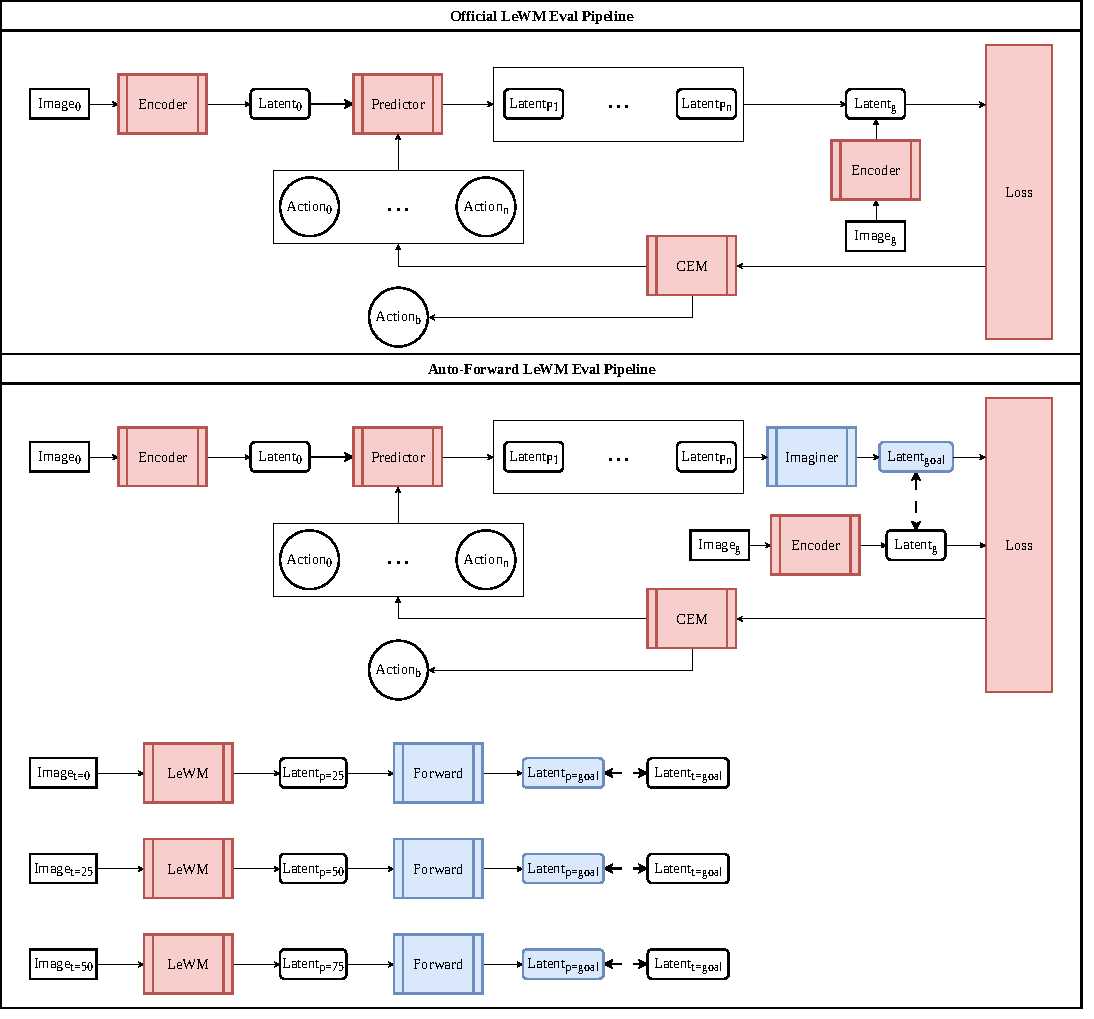
\includegraphics[width=\linewidth]{figures/fig_has_evaluation.pdf}
\caption{\textbf{A longer scoring view for a short action plan.}
The action-conditioned predictor produces an endpoint at $e+H$.
For a later goal at offset $o$, HAS applies the shared Forward map
across the remaining action blocks and evaluates the extended
representation against the goal embedding. The diagram depicts
$o>e+H$; at later replans the extension decreases to zero.}
\label{fig:overview}
\end{figure}

\section{Related Work}
\label{sec:related}

Latent world models provide compact predictive interfaces for visual
control~\citep{hafner2019planet,hafner2020dreamer,hansen2022tdmpc}.
Reward-free goal reaching uses these interfaces to evaluate progress
toward observations specified after training. PLDM learns latent
dynamics from offline trajectories~\citep{sobal2025rewardfree};
DINO-WM predicts pretrained visual features~\citep{zhou2025dinowm};
and LeWM jointly trains the encoder and
predictor~\citep{lewm2026}. Their use of latent prediction motivates
the question of how its temporal coverage relates to the goals
against which candidate actions are evaluated.

Longer-term coverage can be built into prediction and search.
Variable-length world models condition predictions on action
sequences of different durations~\citep{du2026vlwm}, while
hierarchical world models use coarse predictions to guide
local planning~\citep{zhang2026hwm}. Learned subgoals provide
another temporal interface: FF-JEPA proposes successive
subgoals with an action-free latent planner~\citep{masip2026ffjepa},
and SAGE conditions action generation on predicted
subgoals~\citep{cheng2026sage}. These approaches extend the
futures available to the planner or guide its proposals.
Evaluating the endpoint of an already generated candidate
offers a complementary opportunity.

The evaluation signal itself also benefits from planning-oriented
structure. Temporal straightening regularizes latent trajectory
curvature to improve distance geometry~\citep{wang2026straightening}.
RC-aux combines multi-horizon prediction with budget-conditioned
reachability correction~\citep{li2026rcaux}. Traj-LeWM learns a
goal-conditioned trajectory cost that complements endpoint
distance~\citep{huang2026trajlewm}, while TRM learns a temporal
pairwise cost for ranking predicted endpoints against
goals~\citep{li2026trm}. These methods connect temporal,
geometric, and path information with action selection.

HAS focuses on the time-indexed representation supplied to the
endpoint comparison. Its action-free Forward map connects to
latent subgoal prediction~\citep{masip2026ffjepa}, and its scoring
role connects to planning-oriented
costs~\citep{li2026trm,huang2026trajlewm}. HAS applies the shared
map after each action-conditioned candidate rollout and selects
its depth from the remaining gap to the goal. The resulting
temporal extension preserves Euclidean comparison while
giving each short endpoint a longer-horizon scoring view.

\section{Problem Setup}
\label{sec:setup}

Let $x_t$ be an image observation at environment step $t$, with
embedding $z_t=E(x_t)\in\mathbb{R}^d$.
An action block contains $b$ consecutive environment actions.
The predictor $P$ uses recent latent observations and action blocks
to estimate the next latent, and a candidate sequence of $h$ blocks
covers a planning span $H=hb$. We use $b=5$ and default $h=5$,
giving $H=25$ environment steps. All time indices below are relative
to the initial observation; one transition of $P$ or the Forward
imaginer corresponds to one action block.

A goal image is sampled at offset $o$ from the initial observation
and encoded as $z_g=E(x_o)$. After $e$ environment steps of execution,
the planner evaluates candidate sequences $a^{(n)}_{0:h-1}$.
Their predicted endpoints are
\begin{equation}
\hat z^{(n)}_{e+H}
=P^{(h)}(z_e,a^{(n)}_{0:h-1}),
\label{eq:predict-endpoint}
\end{equation}
where $P^{(h)}$ denotes autoregressive prediction with the recent
latent and action context suppressed for clarity. LeWM assigns
the terminal cost
\begin{equation}
C_{\mathrm{LeWM}}^{(n)}
=\left\|\hat z^{(n)}_{e+H}-z_g\right\|_2^2.
\label{eq:lewm-cost}
\end{equation}

When $o-e>H$, the candidate endpoint and goal occupy different
positions on this time axis, separated by $o-e-H$ environment
steps. The current action sequence determines progress up to
$e+H$, while reaching the goal involves further evolution.
HAS uses the remaining gap to determine how far to extend the
candidate's representation for scoring. This separates the span
of action-conditioned search from the temporal view used to
evaluate its outcome.

\section{Horizon-Aligned Scoring}
\label{sec:method}

\subsection{Scoring beyond the planning span}
\label{sec:alignment}

HAS learns a deterministic map
$F:\mathbb{R}^d\rightarrow\mathbb{R}^d$ representing one action
block of latent evolution. At elapsed time $e$, it selects depth
\begin{equation}
k(e,o)=\max\left(\frac{o-e-H}{b},\,0\right).
\label{eq:depth}
\end{equation}
The evaluated offsets and replanning times make every positive
gap divisible by $b$. With $F^0(z)=z$ and
$F^{j+1}(z)=F(F^j(z))$, the HAS cost is
\begin{equation}
C_{\mathrm{HAS}}^{(n)}
=\left\|F^{k(e,o)}\!\left(\hat z^{(n)}_{e+H}\right)-z_g\right\|_2^2.
\label{eq:has-cost}
\end{equation}
Thus, each candidate is evaluated through a temporally extended
representation of its short-rollout endpoint.

The two predictive stages serve complementary roles.
The action-conditioned rollout captures the immediate consequences
of the candidate sequence. Forward then supplies a learned
continuation from that endpoint, using local evolution observed
in the offline trajectories. Its input is a single latent, so
this continuation summarizes evolution under the data distribution.
The extended representation provides a longer-term scoring view
for selecting the current actions; the controller obtains the
next action sequence through replanning from a fresh observation.

The remaining-gap rule adapts this view as execution advances.
For $o=100$ and $H=25$, replans at $e=0,25,50,75$ use
$k=15,10,5,0$, respectively. Once $e+H\ge o$, the extension
is the identity and Equation~\ref{eq:has-cost} becomes the
LeWM terminal cost. HAS therefore joins extended scoring for
distant goals with direct endpoint scoring near the goal horizon.

\subsection{Learning the Forward imaginer}
\label{sec:imaginer}
\label{sec:lewm}

Forward learns from the local transitions already available to
the world model (Figure~\ref{fig:method}). Each training sample contains four encoded
observations $z_{0:3}=E(x_{0:3})$ separated by one action block;
here the subscripts index blocks within the sample. LeWM
produces $p_{0:2}$, with $p_i$ predicting $z_{i+1}$.
Define the mean squared latent error as
$D(z,z')=\|z-z'\|_2^2/d$. The world-model objective is
\begin{equation}
\mathcal{L}_{\mathrm{LeWM}}
=\frac{1}{3}\sum_{i=0}^{2}D(p_i,z_{i+1})
+0.09\,\mathcal{L}_{\mathrm{SIGReg}}(z_{0:3}),
\label{eq:lewm}
\end{equation}
with batch averaging implicit. SIGReg regularizes the embedding
distribution~\citep{lewm2026}, and both predicted and target
embeddings receive gradients from the prediction term.

The alignment $p_i\approx z_{i+1}$ provides two one-step
examples for Forward: $F(p_0)$ predicts $z_2$ and $F(p_1)$
predicts $z_3$. Writing detached tensors with bars, the step loss is
\begin{equation}
\mathcal{L}_{\mathrm{step}}
=\frac{1}{2}\left[
D(F(\bar p_0),\bar z_2)+D(F(\bar p_1),\bar z_3)\right].
\label{eq:forward-step}
\end{equation}
A second term supervises the composition used during planning:
\begin{equation}
\mathcal{L}_{\mathrm{roll}}
=D(F(F(\bar p_0)),\bar z_3),
\label{eq:forward-roll}
\end{equation}
giving
\begin{equation}
\mathcal{L}_F
=\mathcal{L}_{\mathrm{step}}+\mathcal{L}_{\mathrm{roll}}.
\label{eq:forward-total}
\end{equation}
The step term fits local evolution, while the recursive term
trains Forward to consume its own output over two transitions.
Both draw supervision from the same four-observation sample.

Inputs and targets are detached at the interface to Forward,
so the direct gradients of $\mathcal{L}_F$ enter only $F$.
The Forward objective has unit weight in training.
We implement $F$ as a small residual MLP, with architectural
and optimization details in Appendix~\ref{app:implementation}.
Local training produces a shared map that can be repeatedly
applied at the depth selected by Equation~\ref{eq:depth}.

\begin{figure}[tbp]
\centering
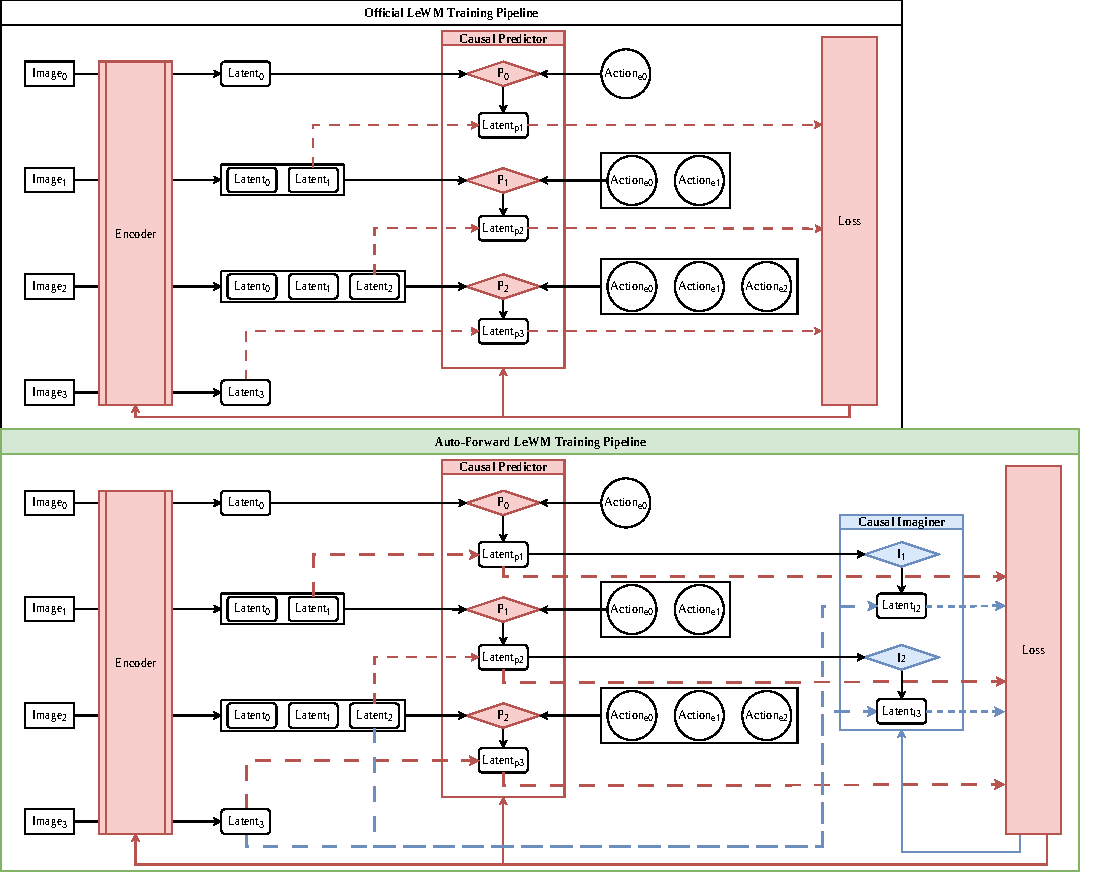
\includegraphics[width=\linewidth]{figures/fig_has_training.pdf}
\caption{Local and recursive supervision for Forward.
LeWM predicts $p_i\approx z_{i+1}$ from the four-observation
training window. Detached predictor outputs supervise the
shared Forward map through $F(p_0)\rightarrow z_2$,
$F(p_1)\rightarrow z_3$, and $F(F(p_0))\rightarrow z_3$.
The schematic $P_i$ instances share the action-conditioned
predictor parameters; each observation interval is one
five-step action block.}
\label{fig:method}
\end{figure}

\subsection{Receding-horizon integration}
\label{sec:planning}

HAS integrates into the Cross-Entropy Method
(CEM)~\citep{rubinstein1999cem} through its candidate cost.
CEM samples sequences of $h$ action blocks, predicts their
endpoints with $P$, and scores their Forward extensions.
It then retains the lowest-cost candidates and fits a diagonal
Gaussian to their empirical moments. After the final update,
the controller executes the receding-horizon prefix of the
mean sequence, advances $e$, and replans from the new
observation. Algorithm~\ref{alg:has-cem} summarizes one call.

\begin{algorithm}[tbp]
\caption{Horizon-Aligned CEM at elapsed time $e$}
\label{alg:has-cem}
{\small
\begin{algorithmic}[1]
\Require current latent and recent context; goal $z_g$; offset $o$
\Require predictor $P$; Forward $F$; block size $b$; span $H=hb$
\Require candidates $N$; elites $M$; updates $J$
\State $k\gets\max((o-e-H)/b,0)$
\State $(\mu_0,\sigma_0)\gets\Call{InitializeCEM}{h}$
\For{$j=1,\ldots,J$}
    \State $A^{(1:N)}\gets\Call{Sample}{\mu_{j-1},\sigma_{j-1},N}$
    \ForAll{$n\in\{1,\ldots,N\}$}
        \State $\hat z^{(n)}_{e+H}\gets P^{(h)}(z_e,A^{(n)})$
        \State $\tilde z^{(n)}\gets F^k(\hat z^{(n)}_{e+H})$
        \State $c_n\gets\|\tilde z^{(n)}-z_g\|_2^2$
    \EndFor
    \State $\mathcal{I}_j\gets\Call{Elite}{c_{1:N},M}$
    \State $(\mu_j,\sigma_j)\gets
        \Call{Moments}{\{A^{(n)}:n\in\mathcal{I}_j\}}$
\EndFor
\State \Return $\mu_J$
\end{algorithmic}
}
\end{algorithm}

For each candidate, HAS adds $k$ evaluations of the residual
MLP to the $h$-block action-conditioned rollout.
The additional Forward computation scales linearly with
recursion depth and candidate count, and decreases as the
goal horizon approaches. The optimized action sequence
retains its length of $h$ blocks.

\section{Experiments}
\label{sec:exp}

\subsection{Experimental setup}

We evaluate whether horizon-aligned scoring improves long-offset
goal reaching and how its recursion depth contributes to that
improvement. PushT~\citep{florence2022ibc},
TwoRoom~\citep{sobal2025rewardfree}, and
Reacher~\citep{lewm2026} provide visual control settings involving
object manipulation, navigation, and reaching.
For each task, we use one epoch-$10$ checkpoint and compare
the LeWM terminal score with HAS on the same world model.
Ten evaluation groups, indexed by seeds $42$--$51$, contain
$50$ episodes each. Methods share the sampled starts and
goals within each task, offset, and group. Reported means and
standard deviations summarize these ten group-level success
rates and measure evaluation variability for the trained model.

Goal offsets are $o\in\{25,50,75,100\}$ environment steps,
with an interaction budget of $2o$ and the success criterion
defined by each environment. The default LeWM and HAS
configurations use $b=5$ and $h=5$, giving $H=25$, and execute
$25$ steps before replanning. To compare the scoring extension
with a longer action-conditioned plan, we also evaluate LeWM
at $H=50$, with $h=10$ and a $50$-step execution prefix.
All configurations use $300$ CEM candidates, $30$ elites,
and $30$ updates. The longer-span configuration therefore
changes both prediction span and replanning frequency;
its $o=25$ condition extends beyond the sampled goal time.
Appendices~\ref{app:implementation} and~\ref{app:protocol}
give training and evaluation details.

\subsection{Long-offset goal reaching}
\label{sec:main}

HAS improves mean success across all three tasks at every
evaluated offset beyond the default planning span
(Table~\ref{tab:main}, Figure~\ref{fig:multiseed}).
The improvement is particularly pronounced in TwoRoom, where
success at $o=100$ rises from $16.4\%$ to $70.4\%$.
PushT at $o=50$ improves from $42.8\%$ to $67.8\%$.
These gains establish that a temporal extension of candidate
endpoints can make the same short action-conditioned planner
more effective at reaching distant visual goals.

\begin{figure}[t]
\centering
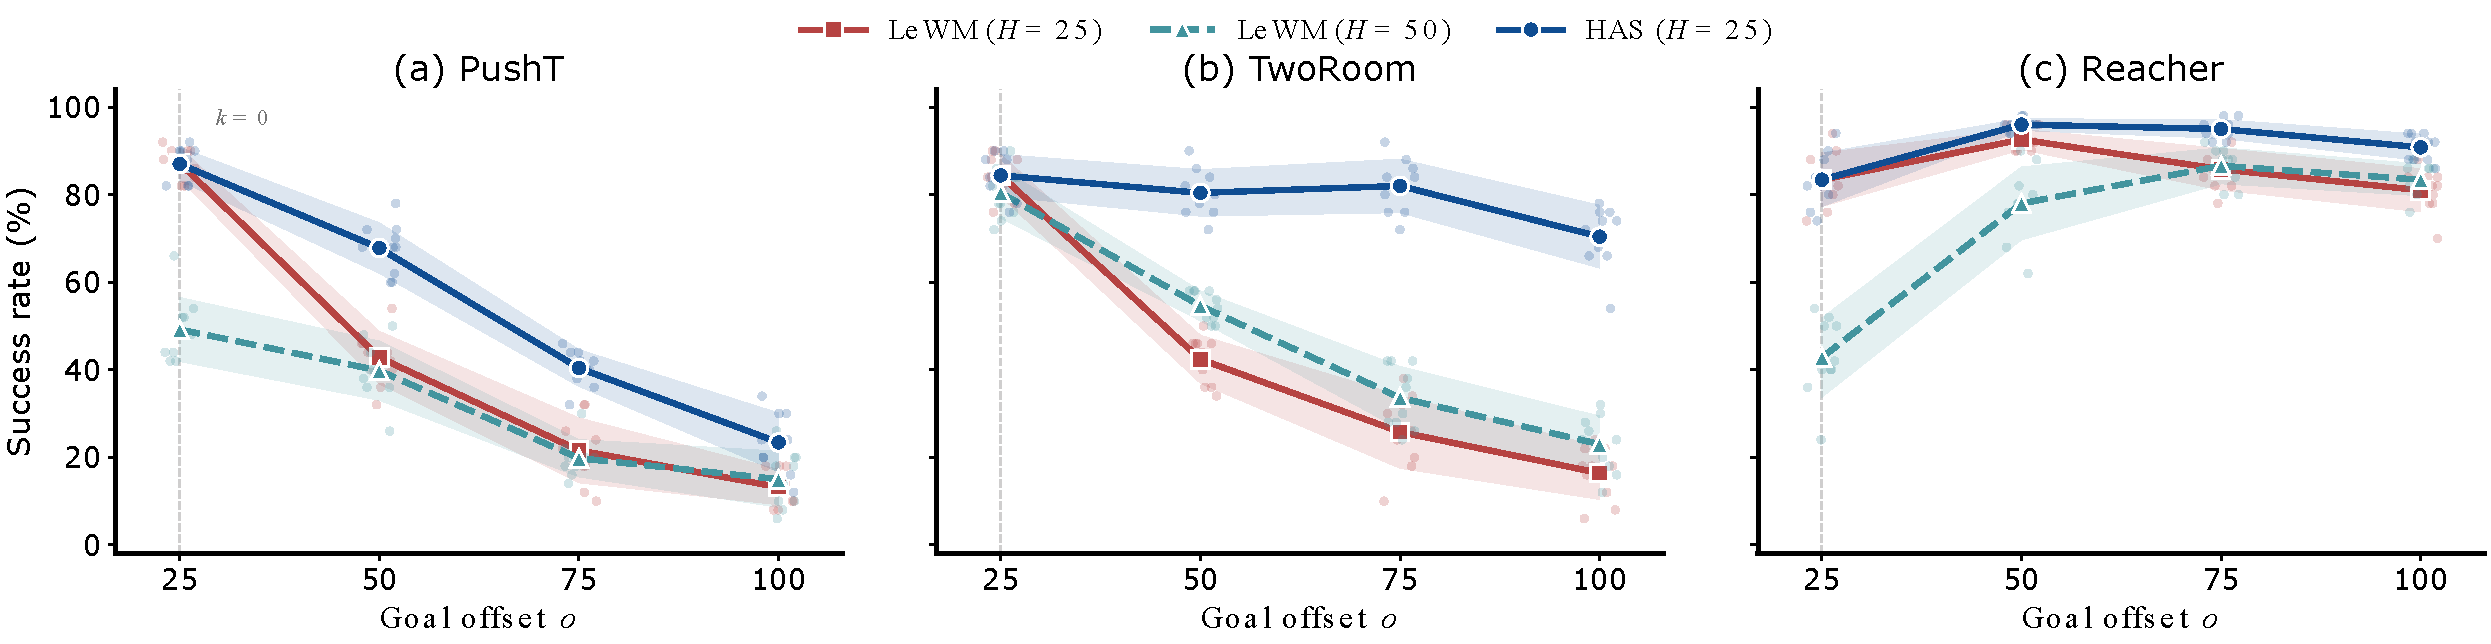
\includegraphics[width=0.98\linewidth]{figures/fig_iclr_multiseed.pdf}
\caption{Goal reaching across temporal offsets. Points are
success rates for evaluation groups of $50$ episodes; lines
and shaded bands give the mean and standard deviation over
ten groups using one checkpoint per task. The dashed line
marks the default planning span $H=25$, where HAS uses $k=0$.}
\label{fig:multiseed}
\end{figure}

\begin{table}[t]
\caption{Success rate (\%; mean $\pm$ std over $10$ evaluation
groups). Bold marks the highest mean for each task and offset.
$^\dagger$LeWM with $H{=}50$, so the $o{=}25$ column is a
non-primary overshoot condition.}
\label{tab:main}
\begin{center}
\small
\begin{tabular}{llcccc}
\toprule
Task & Method & $o{=}25$ & $o{=}50$ & $o{=}75$ & $o{=}100$ \\
\midrule
PushT & LeWM ($H{=}25$)
  & $\mathbf{87.2{\pm}3.6}$ & $42.8{\pm}6.0$ & $21.6{\pm}7.4$ & $13.2{\pm}4.0$ \\
 & LeWM ($H{=}50$)
  & $49.2{\pm}7.3^\dagger$ & $39.8{\pm}6.8$ & $19.8{\pm}4.3$ & $15.0{\pm}6.4$ \\
 & HAS ($H{=}25$)
  & $87.0{\pm}3.8$ & $\mathbf{67.8{\pm}5.8}$ & $\mathbf{40.4{\pm}4.2}$
  & $\mathbf{23.4{\pm}6.7}$ \\
\midrule
TwoRoom & LeWM ($H{=}25$)
  & $\mathbf{84.4{\pm}4.8}$ & $42.4{\pm}5.5$ & $25.8{\pm}8.3$ & $16.4{\pm}6.0$ \\
 & LeWM ($H{=}50$)
  & $80.4{\pm}5.7^\dagger$ & $54.6{\pm}3.4$ & $33.6{\pm}7.2$ & $23.0{\pm}6.4$ \\
 & HAS ($H{=}25$)
  & $\mathbf{84.4{\pm}4.8}$ & $\mathbf{80.4{\pm}5.3}$ & $\mathbf{82.0{\pm}6.1}$
  & $\mathbf{70.4{\pm}7.2}$ \\
\midrule
Reacher & LeWM ($H{=}25$)
  & $\mathbf{83.4{\pm}6.1}$ & $92.6{\pm}2.3$ & $85.8{\pm}4.8$ & $81.0{\pm}4.9$ \\
 & LeWM ($H{=}50$)
  & $42.8{\pm}9.1^\dagger$ & $78.0{\pm}8.3$ & $86.6{\pm}4.1$ & $83.4{\pm}3.7$ \\
 & HAS ($H{=}25$)
  & $\mathbf{83.4{\pm}6.1}$ & $\mathbf{96.0{\pm}1.3}$ & $\mathbf{95.0{\pm}2.2}$
  & $\mathbf{90.8{\pm}3.0}$ \\
\bottomrule
\end{tabular}
\end{center}
\end{table}

The cross-task pattern indicates that the value of extended
scoring depends on the control setting. Navigation in TwoRoom
requires intermediate progress through a passage, making a
later view of an endpoint especially useful. Reacher already
has a strong LeWM baseline, yet HAS improves its long-offset
performance as well. Contact-rich PushT benefits from the
same scoring design but remains difficult at the longest
offset. Taken together, the results support temporal
extension as a useful scoring operation across these settings,
with the largest gains where short-term proximity provides
a limited view of task progress.

A longer action-conditioned plan is a natural alternative
way to look farther ahead. In the evaluated $H=50$
configuration, LeWM remains below HAS at every offset of
$50$ steps or more. For example, TwoRoom at $o=100$ reaches
$23.0\%$ with this longer-span configuration, compared with
$70.4\%$ under HAS. Extending the scoring representation
therefore provides a practical benefit beyond that obtained
by the tested increase in planning span. This comparison
motivates a closer examination of how the Forward extension
itself should be scheduled.

\subsection{The role of alignment depth}
\label{sec:ablation}

The usefulness of Forward depends on how far it is applied.
We compare the remaining-gap rule with fixed depths
$k\in\{0,5,10,15\}$ on the same ten evaluation groups at
$o\in\{75,100\}$ (Table~\ref{tab:k-depth}). A fixed depth
is applied at every replan, including late in execution when
the dynamic rule has reached zero. This comparison tests
the full depth schedule: the initial extension and its
reduction as the controller approaches the goal horizon.

\begin{table}[t]
\centering
\caption{Success rate (\%; mean $\pm$ std over ten evaluation
groups) under different Forward depths. HAS uses the
remaining-gap rule; fixed $k$ is reapplied at every replan.
The world-model checkpoint, starts, and CEM configuration
are shared within each task and evaluation group.}
\label{tab:k-depth}
{\small
\begin{tabular}{llccccc}
\toprule
Task & $o$ & $k{=}0$ & $k{=}5$ & $k{=}10$ & $k{=}15$ & HAS \\
\midrule
PushT & $75$ & 21.6$\pm$7.4 & 4.0$\pm$2.7 & 0.8$\pm$1.0 & 0.4$\pm$0.8 & 40.4$\pm$4.2 \\
PushT & $100$ & 13.2$\pm$4.0 & 2.6$\pm$1.9 & 0.4$\pm$0.8 & 0.6$\pm$1.0 & 23.4$\pm$6.7 \\
\midrule
TwoRoom & $75$ & 25.8$\pm$8.3 & 66.6$\pm$3.1 & 29.0$\pm$6.1 & 13.6$\pm$3.7 & 82.0$\pm$6.1 \\
TwoRoom & $100$ & 16.4$\pm$6.0 & 76.2$\pm$5.7 & 31.6$\pm$5.5 & 12.8$\pm$2.1 & 70.4$\pm$7.2 \\
\midrule
Reacher & $75$ & 85.8$\pm$4.8 & 83.6$\pm$4.5 & 67.6$\pm$5.1 & 45.6$\pm$6.4 & 95.0$\pm$2.2 \\
Reacher & $100$ & 81.0$\pm$4.9 & 80.6$\pm$5.5 & 71.2$\pm$6.7 & 47.4$\pm$7.4 & 90.8$\pm$3.0 \\
\bottomrule
\end{tabular}

}
\end{table}

Dynamic alignment achieves the highest mean in five of the
six task--offset conditions, making it a strong default
across the tested settings. Fixed deep recursion is
particularly unfavorable in PushT: at $o=75$, HAS reaches
$40.4\%$, while fixed depths of $5$ or more remain at $4.0\%$
or below. Repeated extension alone is therefore insufficient;
adapting its depth during execution is an important part of
the scoring design. The fixed-depth results also make clear
that applying more Forward steps need not improve control.

The strongest fixed setting exceeds HAS in one condition:
TwoRoom at $o=100$ achieves $76.2\%$ with $k=5$, compared
with $70.4\%$ under the dynamic rule. This exception
suggests that the most useful extension also depends on
task evolution and the behavior of recursive predictions.
The remaining-gap rule offers broad performance across
conditions, while the preferred depth can be task-dependent.
At the short-offset boundary, the $k=0$ cost identity in
Section~\ref{sec:alignment} corresponds to matching success
in TwoRoom and Reacher and near-matching success in PushT
($87.2\%$ for LeWM and $87.0\%$ for HAS at $o=25$).

% HAS_TRAIN_SEEDS_PENDING:
% The author confirms 3 training seeds x 3 tasks, with BOTH official
% (LeWM) and HAS evaluations at offsets 25/50/75/100 for every run.
% Once complete results are supplied, aggregate evaluation groups within
% each run/method, then report mean and sample SD (ddof=1) across runs.
% Compute HAS-minus-official gains within matching training runs.
% Replace tab:main with the paired three-training-seed comparison;
% preserve its current three-way numbers in a separate H=50 control table.
% Update Abstract, Introduction, protocol, main results, and Limitations.
% Move the existing single-checkpoint fig:multiseed to the appendix.
% Add a concise Robustness across training runs subsection and per-run
% appendix table. No pending-result claims or placeholders in the PDF.

\subsection{How temporal extension changes scoring}
\label{sec:score-analysis}

Temporal extension makes intermediate states more comparable to
later goals in the learned latent space. To examine this operation,
we compare the distance from an observed endpoint $z_H$ to its
later goal $z_g$ with the distance after applying Forward:
$\|z_H-z_g\|_2$ versus $\|F^k(z_H)-z_g\|_2$.
The diagnostic uses $400$ evaluation-disjoint trajectory windows
per task, with $H=25$ and $(k,o)\in\{(5,50),(10,75),(15,100)\}$.
Using encoder endpoints exposes the transformation performed by
Forward directly; Appendix~\ref{app:analysis} gives the sampling
protocol.

\begin{figure}[tbp]
\centering
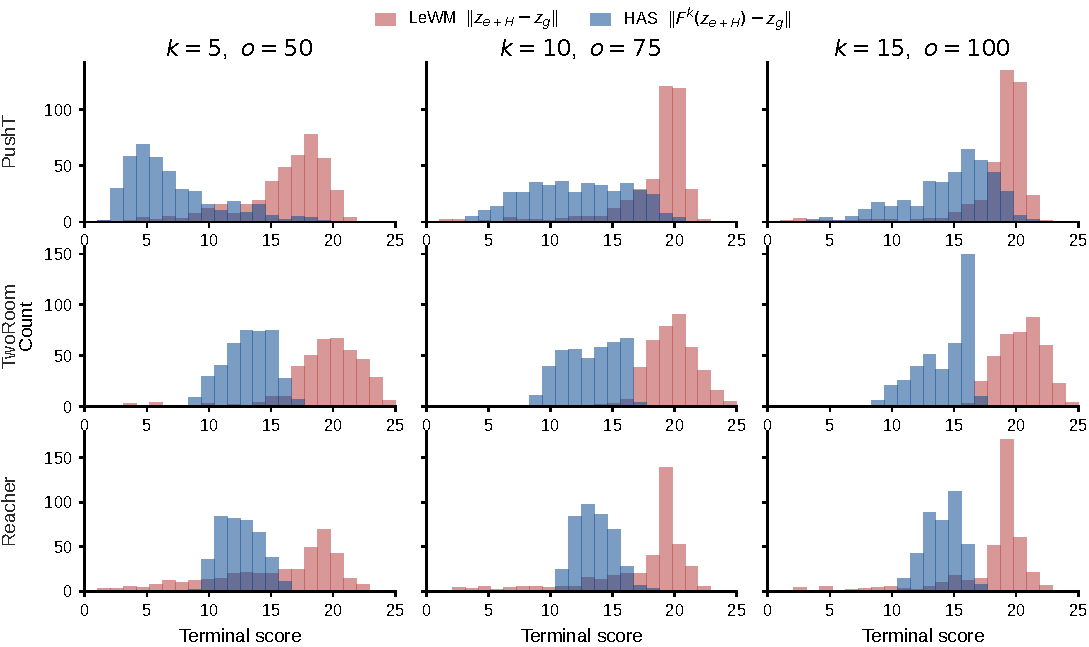
\includegraphics[width=\linewidth]{figures/fig_has_score_contrast.pdf}
\caption{Endpoint-to-goal distances on $400$ evaluation-disjoint
trajectory windows per task. Direct distances use encoder
latents at $H=25$ and the goal offset $o$; extended distances
apply $k=(o-H)/b$ Forward steps to the encoder endpoint.
The horizontal axis gives Euclidean distance (the square
root of the planning cost), and the vertical axis counts
windows.}
\label{fig:score}
\end{figure}

The extended representations generally occupy a lower
endpoint-to-goal distance range (Figure~\ref{fig:score}).
This pattern shows how locally learned evolution can bridge part
of the representational gap between an intermediate state and
a later goal. In PushT, the direct and extended distributions
overlap more at the longest offset, consistent with the greater
difficulty of recursive extension in this setting.
The diagnostic makes the representational effect of HAS visible,
while the closed-loop comparisons establish its control benefit.
Its scope is the transformation of observed endpoint distances;
candidate-ranking accuracy is a separate property.
The paired executions below connect this scoring perspective
to intermediate progress during control.

\subsection{Planning behavior}
\label{sec:analysis}

Useful short-term actions can first establish intermediate
progress before the goal configuration becomes locally
attainable. The paired executions in
Figure~\ref{fig:process} illustrate this distinction.
In TwoRoom, the HAS trajectory advances toward and through
the passage, while the LeWM trajectory remains on the
starting side. In PushT, the HAS sequence first changes the
pusher's position and subsequently brings the object toward
the target configuration. These trajectories connect the
scoring perspective to control behavior: candidate endpoints
can be valuable because of the progress that follows them.

\begin{figure}[tbp]
\centering
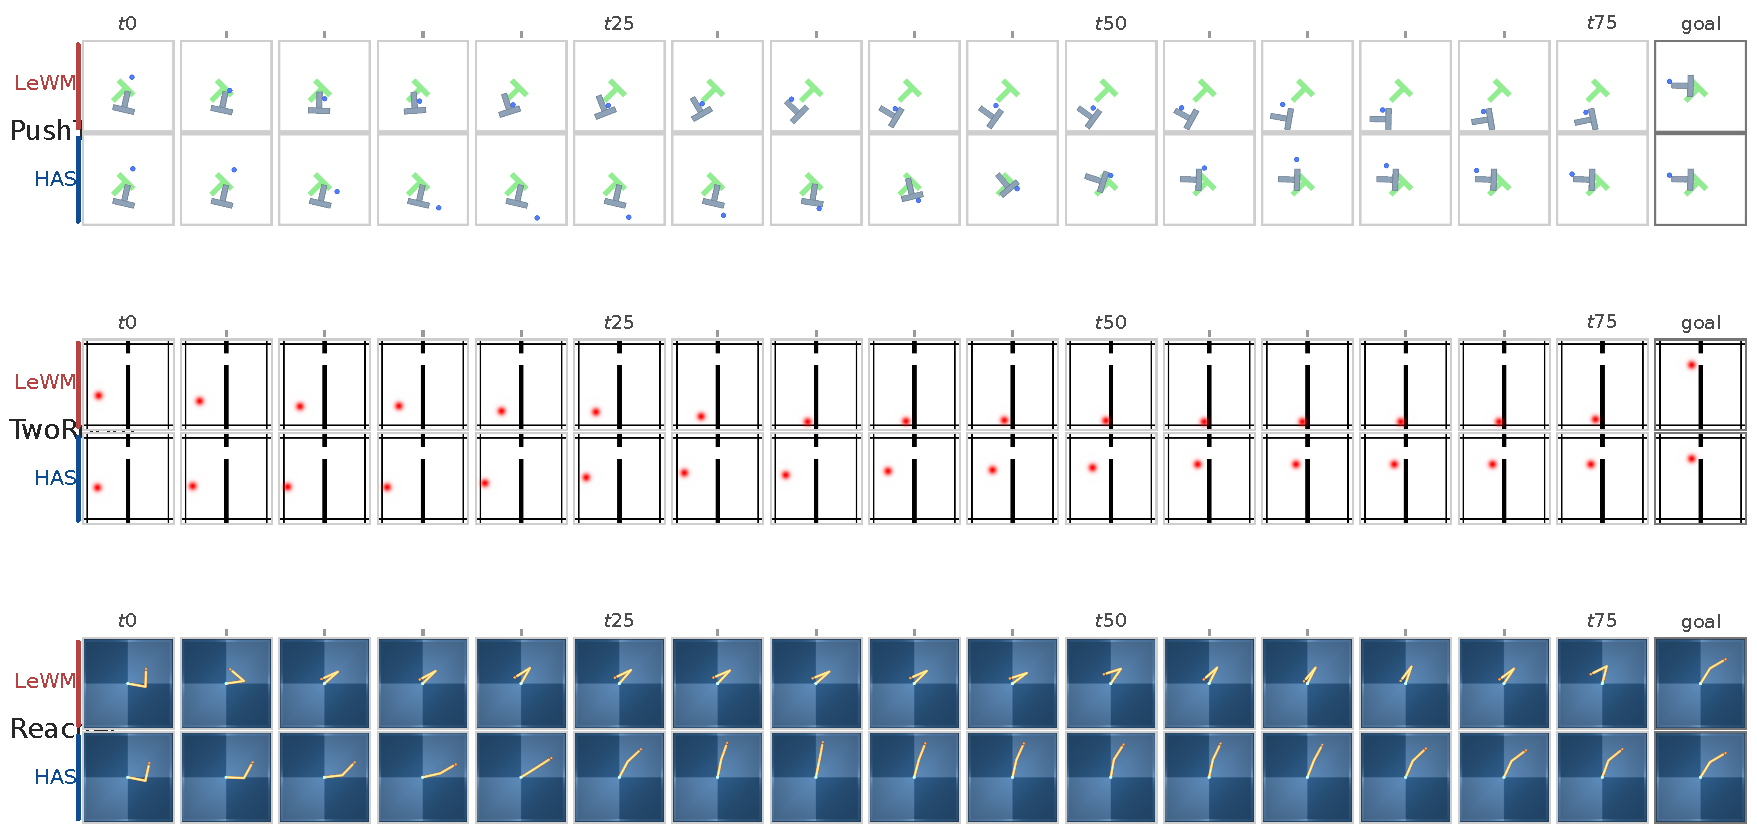
\includegraphics[width=\linewidth]{figures/fig_has_process.pdf}
\caption{Paired executions from one shared start per task at
goal offset $o=75$, using LeWM and HAS with $H=25$.
Frames are spaced by one action block ($5$ environment steps);
the last column is the visual goal. HAS succeeds on these
selected starts, while LeWM fails under the environment
success criterion.}
\label{fig:process}
\end{figure}

\subsection{Limitations}
\label{sec:limits}

HAS uses the known goal offset to select its recursion depth,
so tasks specified solely by a goal image require an
additional estimate or choice of temporal scale.
An action-free deterministic map summarizes local evolution
under the training distribution; long recursions can
accumulate error or compress multiple possible continuations
into an unhelpful representation. These issues are especially
relevant to contact-rich control, as reflected in the
remaining difficulty of long-offset PushT.
The reported comparisons cover three simulated tasks with
one training checkpoint per task; their ten evaluation groups
measure variability in evaluation. The $H=50$ control examines
one longer-span configuration, and further spans or compute
budgets could change the relative performance.

\section{Conclusion}
\label{sec:concl}

The time scale of candidate evaluation matters when a visual
world model plans toward goals beyond its prediction span.
HAS gives short action-conditioned endpoints a longer scoring
view through a locally trained Forward imaginer and a
remaining-gap recursion rule. Across PushT, TwoRoom, and
Reacher, this design improves long-offset goal reaching and
exceeds the evaluated longer-span LeWM configuration.
The depth comparison further demonstrates the value of
adapting the extension during execution.
Together, these findings identify temporal extension at the
scoring interface as a useful way to connect local predictive
models with longer-horizon control, and motivate treating
scoring depth as an explicit component of world-model planning.

\subsection*{AI use statement}

We used generative AI tools for implementation assistance,
literature-checking assistance, structural planning, interpretation
of existing results, drafting, and language editing. The authors are responsible for
verifying the experimental results, references, and claims,
and for the final content of the manuscript.

\subsection*{Ethics statement}

This work evaluates visual goal-conditioned control in
simulated manipulation, navigation, and reaching tasks.
The experiments involve simulated observations and actions,
with no human-subject or personal-data collection.
Deployment on physical systems would require separate
validation of control safety and failure recovery.

\subsection*{Reproducibility statement}

Sections~\ref{sec:setup} and~\ref{sec:method} specify the time
scales, training objectives, gradient boundaries, recursion
rule, and planning algorithm.
Appendix~\ref{app:implementation} gives the Forward architecture
and optimization settings, and Appendix~\ref{app:protocol}
describes the paired evaluation and aggregation procedure.
The table captions identify the statistical units used for
the reported results. Appendix~\ref{app:analysis} documents
the sampling and computations of the offline scoring
diagnostic.


\bibliography{iclr2027_conference}
\bibliographystyle{iclr2027_conference}

\clearpage
\appendix
\section{Training and implementation}
\label{app:implementation}

Each training window contains four observations sampled every
five environment steps. Predictor outputs $p_0,p_1,p_2$ align
with encoder latents $z_1,z_2,z_3$, respectively. Forward uses
$p_0$ and $p_1$ as one-step inputs with targets $z_2$ and $z_3$;
its recursive example maps $p_0$ to $z_3$ through two
applications. Figure~\ref{fig:method} summarizes this
supervision. All instances of $F$ share parameters, and
the training losses average squared errors across latent
dimensions and batch examples.

Forward operates on $192$-dimensional latents using two
residual MLP blocks. Each block applies LayerNorm, a linear
expansion to width $768$, GELU, and a linear projection back
to $192$ dimensions before the residual addition. A final
LayerNorm and linear projection produce the output.
The input consists of one latent representation.
Predictor inputs and encoder targets are detached before
the Forward losses, so their direct gradients update
Forward parameters.

Training uses AdamW with learning rate $5\times10^{-5}$,
weight decay $10^{-3}$, batch size $128$, bfloat16
precision, and global gradient clipping at norm $1.0$.
The LeWM SIGReg coefficient is $0.09$. Both the Forward
step and recursive terms have coefficient $1.0$, as does
the complete Forward objective in the training loop.
The reported comparisons use the epoch-$10$ checkpoint
from one training run per task.

The checkpoint-producing implementation also includes a
parameter-disjoint backward auxiliary head.
Its inputs and targets are detached, so its loss supplies
direct gradients only to that head.
HAS evaluation uses the Forward scoring path described
in Section~\ref{sec:method}.

\section{Evaluation protocol}
\label{app:protocol}

CEM samples $300$ candidates per update, retains the $30$
lowest-cost candidates, and performs $30$ distribution
updates with initial variance scale $1.0$. The default
LeWM and HAS configurations plan $h=5$ action blocks
and execute a prefix of five blocks before replanning.
The longer-span LeWM configuration uses ten blocks for
both planning and execution, retaining the same candidate,
elite, and update counts. These settings correspond to
$25$ and $50$ environment steps, respectively, subject
to the episode termination and interaction budget.

Goals are drawn at offsets $o\in\{25,50,75,100\}$
environment steps, with budget $2o$. For each task and
offset, evaluation groups $42$--$51$ each contain
$50$ episodes. All methods reuse the corresponding
start manifests, including initial states and sampled goals.
Success follows the task environment's criterion.
We compute one success rate per group and configuration,
then report the mean and standard deviation of these ten
rates. The fixed-depth comparison uses the same protocol
and the same checkpoint within each task.

The dynamic rule uses
$k=\max((o-e-H)/b,0)$, with every positive remainder
divisible by $b$ in the evaluated configurations.
When $k=0$, the Forward map is bypassed.
For fixed-depth evaluation, the specified depth overrides
this rule at every replanning step, including steps after
the dynamic extension would have stopped.
The ablation therefore evaluates a depth schedule over
the whole execution.

\section{Scoring diagnostic protocol}
\label{app:analysis}

Figure~\ref{fig:score} uses $400$ offline trajectory windows
per task, sampled after excluding every episode listed in
the ten evaluation-group manifests. Each window covers at
least $100$ environment steps and is encoded using the same
epoch-$10$ checkpoint as the control experiments.
For each window, $z_H$ is the encoder representation at
$H=25$ and $z_g$ corresponds to offset $o\in\{50,75,100\}$.
The Forward depth is $k=(o-H)/b$ with $b=5$.
The plotted quantities are Euclidean norms; the planner uses
their squares. This diagnostic evaluates encoded observations
and their Forward extensions, with no CEM candidate search.

\end{document}
